\chapter{Provázaní Backendu a Frontendu, API}

\section{Dokumentace online}
Aktuální dokumentace, tak aby mohla být časem aktualizována a mohli do ní
být připisovány další věci, se nachází na webu
\href{http://quest.ms.mff.cuni.cz/prak/api/documentation}{.../prak/api/documentation}.
\\
Dokumentace je rozdělena na dvě části.
\\
\\
\textbf{První část} popisuje volání API.\\
Každá metoda (GET, POST atd.) má svůj vlastní účel,
jež je popsán uvnitř url, a další možné parametry.
Spolu s formátem requestu je zde i formát odpovědi.
Podle kódu zjistíme, jestli byl náš požadavek úspěšný.
Kódy jsou standardní podle "http status codes".
\begin{itemize}
	\item \textbf{2xx} Všechno dopadlo dobře
	\item \textbf{4xx} Chyba je na straně klienta
	\item \textbf{5xx} Chyba je na straně serveru
\end{itemize}
V případě úspěchu (kód 200 - OK) se odešle odpověď na dotaz nebo
prázdné tělo, pokud request neměl za funkci něco vracet.
V případě neúspěchu pak v odpovědi najdeme zprávu o chybě, která nastala.
Obvykle to u kódu 500 bývá odeslání duplicitního záznamu.
\\
\\
\textbf{Druhá část} popisuje strukturu schémat jednotlivých modelů.\\
Jelikož databáze má datové formáty, zatímco JSON soubor ne (nebo alespoň ne tak rozsáhlé),
musí i odesílaná data mít správný formát, nebo alespoň být validní po automatickém
přetypovaní.
Schéma tvoří JSON objekt, jež toto schéma popisuje.
Pokud je datový typ položky objekt buď se opravdu jedná o objekt, nebo
se jedna pouze o upřesněni datového typu.
Klíčovými slovy jsou:
\begin{itemize}
	\item \textbf{type}: datový typ
	\item \textbf{required}: true, pokud je tato položka povinná
	\item \textbf{unique}: true, pokud se zadaná hodnota nesmí shodovat s již existující položkou v DB
	\item \textbf{ref}: název schématu, na který se ID odkazuje
	\item \textbf{refPath}: speciální ref, umožnující uživateli zadat i název schématu, vůči kterému se odkazuje
\end{itemize}
Pokud je hodnota pouze string, pak je tato hodnota datovým typem.

\subsection{Software pro online dokumentaci}
Pro možnost stažení dokumentace a prohlížení offline, je vše zabaleno do jediného html souboru.
Uvnitř je zdrojový kód programu, jež vykresluje stránku a zároveň data dokumentace.
\\
Program vykresluje veškeré položky s daty dokumentace.
Bloky zdrojových kódu jsou vysázený fontem monospace a obarvený, aby uživateli
poskytly rychlejší orientaci v kódu.
\\
\begin{figure}[H]
	\centering
	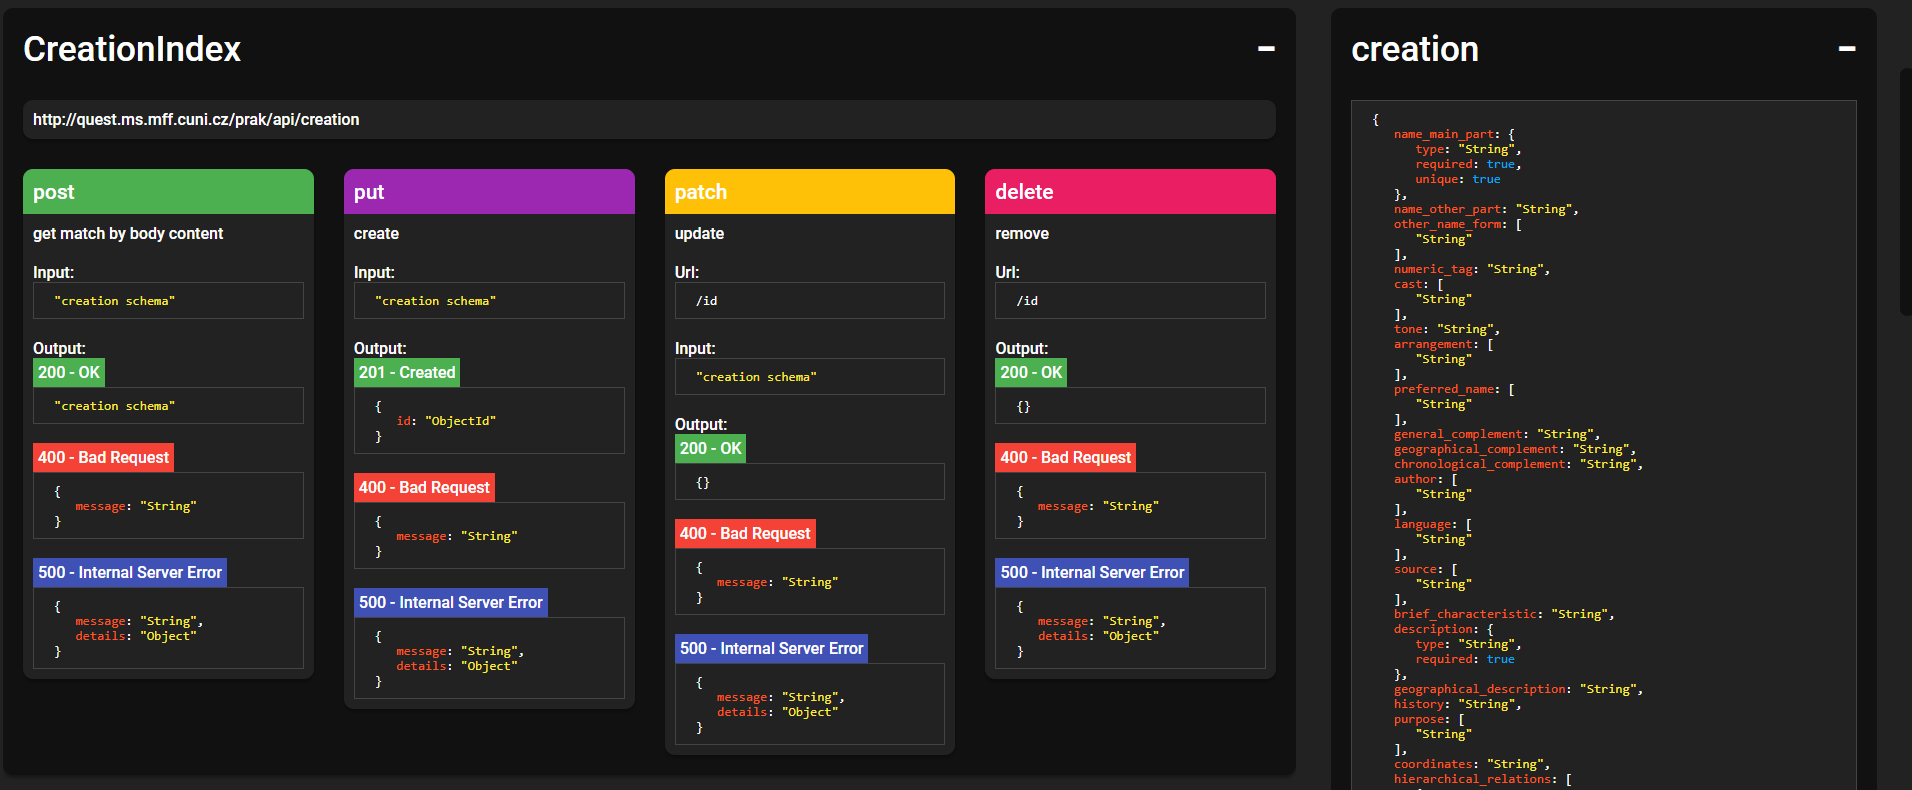
\includegraphics[width=\linewidth]{img/documentationPreview.PNG}
	\caption{Dokumentace API jako webová stránka}
\end{figure}


\section{Backend}
Na backendu je spuštěný express server (bežící pod nodejs), který
zachytává requesty s url \texttt{...prak/api/...} .
Podle cesty, jež je uvedena za /api se request předává
příslušnému routeru. Výjimku tvoří adresa .../api/documentation, která
rovnou přeposílá soubor s dokumentaci a není tedy pro získaní dokumentace
třeba rozumět systému requestů hlouběji.
\\
\\
Při převzetí requestu jedním z mnoha routerů, se porovnává
typ requestu (POST, PUT atd.) a případné detaily cesty v url.
Při plném nalezení shody se provede ověření práv, pokud je to potřeba.
Pokud request má požadovaná oprávnění, je provedena příslušná funkce
a uživateli je vrácena odpověď případně potvrzení o úspěchu.
V případě, že request nemá příslušná oprávnění, je vrácen kód 401.
V případě, že se na serveru něco pokazí, vrátí se kód 400, nebo 500, podle typu problému.

\section{API}
API je přístupné na adrese \texttt{quest.ms.mff.cuni.cz/prak/api/...} .

\subsection{Autentifikace}
S každým requestem přichází v hlavičce i cookie, ten pro
autentifikaci se jmenuje "sessionID".
Podle něj se najde příslušný uživatel a porovnají se jeho práva a
práva potřebná pro vykonání požadované funkce. Pokud jsou práva nedostatečná,
vrátí se odpověď s kódem 401, v případě správného oprávnění router vykoná funkci,
jež danému requestu přísluší a pokud se nepokazí nic jiného, vrátí validní odpověď.

\section{Frontend a volaní API}
Jelikož je celý projekt zamýšlen jako webová aplikace, nejstandardnější použití
je volání API pomocí JS funkce \textit{fetch()}, což je pouze technický alias pro XMLHttpRequest.
Ale je možné jej volat jakkoliv jinak, dokud to bude validní http request.

\subsection{Fetch}
Dokumentace metody: \href{https://developer.mozilla.org/en-US/docs/Web/API/Fetch_API}{developer.mozilla.org}
\\
Příklad použití:
\\
\begin{lstlisting}[language=JavaScript]
	const url = "/prak/api/metadata" 
	fetch(url, {
		method: "POST",
		headers: { "Content-Type": "application/json" },
		body: JSON.stringify({ "name": "..." }),
	})
	.then(response => {
		if(!response.ok) throw response
		return response.json()
	})
	.then(response => {
		console.log(response)
	})
	.catch(error => {
		console.error(error)
	})
\end{lstlisting}

\subsection{Existující programy pro práci a testovaní API}
Příklad volání pomocí programu Insomnia:
\begin{figure}[H]
	\centering
	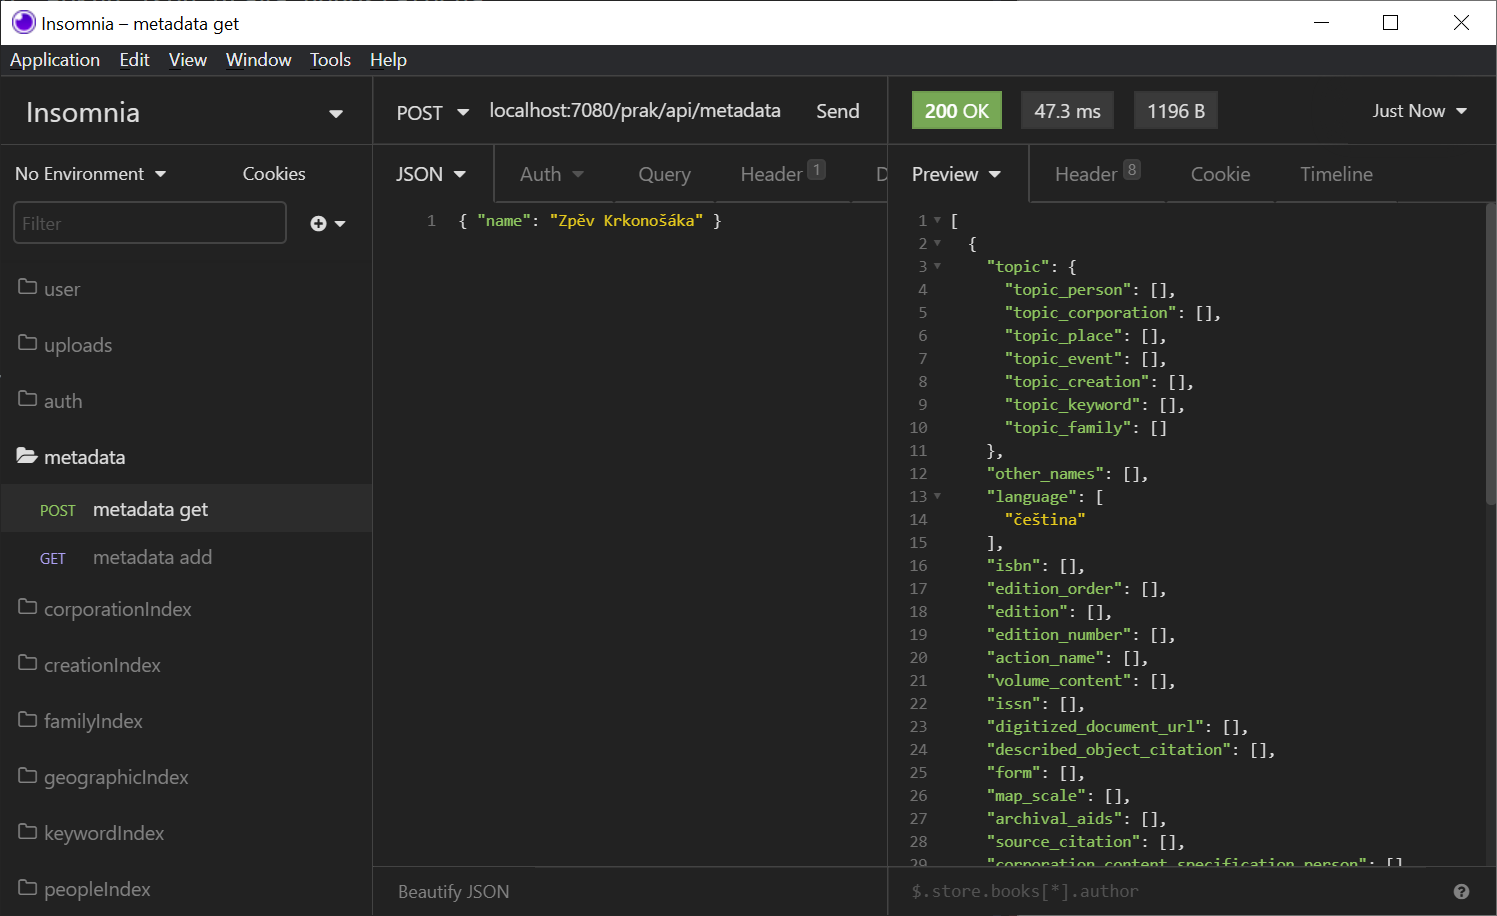
\includegraphics[width=\linewidth]{img/InsomniaExample.PNG}
	\caption{Program insomnia s vyplněným dotazem pro odeslání požadavku na API}
\end{figure}
